\documentclass[a4paper]{cernatsnote}
\usepackage{graphicx}
\usepackage{listings}
\usepackage{caption}
\usepackage{listings}
\usepackage{parskip}
\usepackage{hyperref}
\usepackage{caption}
\usepackage{subcaption}

\email{haroon.rafique@cern.ch}

\title{PTC-PyORBIT SIS18 Benchmark}
\documentlabel{CERN-ATS-Note-2018-??? TECH}

\author{Haroon Rafique / BE-ABP}
\keywords{PyORBIT, Space Charge, SIS18, Benchmark}
\makeindex

\def \gsiSISpage {\href{https://web-docs.gsi.de/~giuliano/research_activity/trapping_benchmarking/main.html}{https://web-docs.gsi.de/~giuliano/research\_activity/trapping\_benchmarking/main.html}}

\begin{document}
	
\maketitle % this produces the title block

\begin{abstract}
	Giuliano Franchetti's SIS18 benchmark has been performed with the PTC-PyORBIT code, the results are detailed in this report.
\end{abstract}

%%%%%%%%%%%%%%%%%%----------------------------------------------------------------------------------------
%% INTRODUCTION %%
%%%%%%%%%%%%%%%%%%----------------------------------------------------------------------------------------	
\section{Introduction}
\label{sec:intro}

Details of the SIS18 benchmark can be found at:
\gsiSISpage

These instructions are repeated and expanded upon here. 
	
%% Setup %%
%%%%%%%%%%%%%%------------------------------------------------------------------------------------------			
\section{Simulation Setup}

The parameters in table~\ref{tab:parameters16} are used in steps 1 - 6, and the changes in table~\ref{tab:parameters79} are used in steps 7 - 9.

\begin{table}
	\begin{center}
		\begin{tabular}[!b]{|l|c|c|c|}
			\hline
			\textbf{Parameter} & \textbf{Symbol} & \textbf{Value} & \textbf{Unit} \\
			\hline
			\textbf{Sextupole Strength} & $K_2$ & 0.2 & $m^{-2}$ \\
			\textbf{Maximum Tuneshift} & $\Delta Q_x$ & 0.1 & $-$ \\
			\textbf{Horizontal Transverse Size (rms)} & $X_{rms}$ & 5 & $mm$ \\
			\textbf{Vertical Transverse Size (rms)} & $Y_{rms}$ & 5 & $mm$ \\
			\textbf{Longitudinal Size (rms)} & $Z_{rms}$ & 40.35 & $m$ \\
			\textbf{Horizontal Geometric Emittance (2 $\sigma$)} & $\epsilon_x$ & 12.57 & $mm~mrad$ \\
			\textbf{Vertical Geometric Emittance (2 $\sigma$)} & $\epsilon_y$ & 9.30 & $mm~mrad$ \\
			\textbf{One Synchrotron Oscillation} & $N_{synch}$ & 15000 & $turns$ \\
			\textbf{Bunch Length (4 $\sigma_z$)} & $\tau$ & 3472.7 & $ns$ \\
			\textbf{Kinetic Energy} & $E_k$ & 11.4 & $MeV/u$ \\
			\textbf{Transition Gamma} & $\gamma_t$ & 5 & $-$ \\
			\textbf{Momentum Spread (3 $\sigma$)} & $\frac{\Delta p}{p}$ & 2.5$\cdot 10^{-4}$ & $-$ \\
			\textbf{Sextupole Strength} & $K_2$ & 0.2 & $m^{-2}$ \\
			\hline
		\end{tabular}
		\caption{Parameters used for the SIS18 benchmark steps 1 - 6.}
		\label{tab:parameters16}
	\end{center}
\end{table}

\begin{table}
	\begin{center}
		\begin{tabular}[!b]{|l|c|c|c|}
			\hline
			\textbf{Parameter} & \textbf{Symbol} & \textbf{Value} & \textbf{Unit} \\
			\hline
			\textbf{Longitudinal Size (rms)} & $Z_{rms}$ & 2.69 & $m$ \\
			\textbf{One Synchrotron Oscillation} & $N_{synch}$ & 1000 & $turns$ \\
			\textbf{Bunch Length (4 $\sigma_z$)} & $\tau$ &  231.51 & $ns$ \\
			\hline
		\end{tabular}
		\caption{Parameter changes used for the SIS18 benchmark steps 7 - 9.}
		\label{tab:parameters79}
	\end{center}
\end{table}

\newpage

\section{Step 1: Benchmarking of the phase space}

The first step is to confirm that the phase space near the 3rd order resonance has the same topology for all codes. We check the orbits up to the border of stability (dynamic aperture). For this test the tunes are $Q_x$ = 4.338, $Q_y$ = 3.2, the Poincar\'{e} section is plot at the beginning of the SIS18 lattice. 

\begin{figure}
        \centering
        \begin{subfigure}{.5\textwidth}
          \centering
          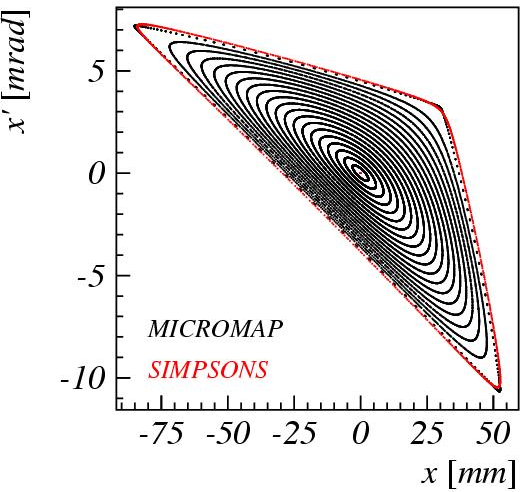
\includegraphics[width=\textwidth]{Step1_phase-space.png}
          \caption{MICROMAP and SIMPSONS.}
          \label{fig:step1_m}
        \end{subfigure}~~~~~~
        \begin{subfigure}{.5\textwidth}
          \centering
          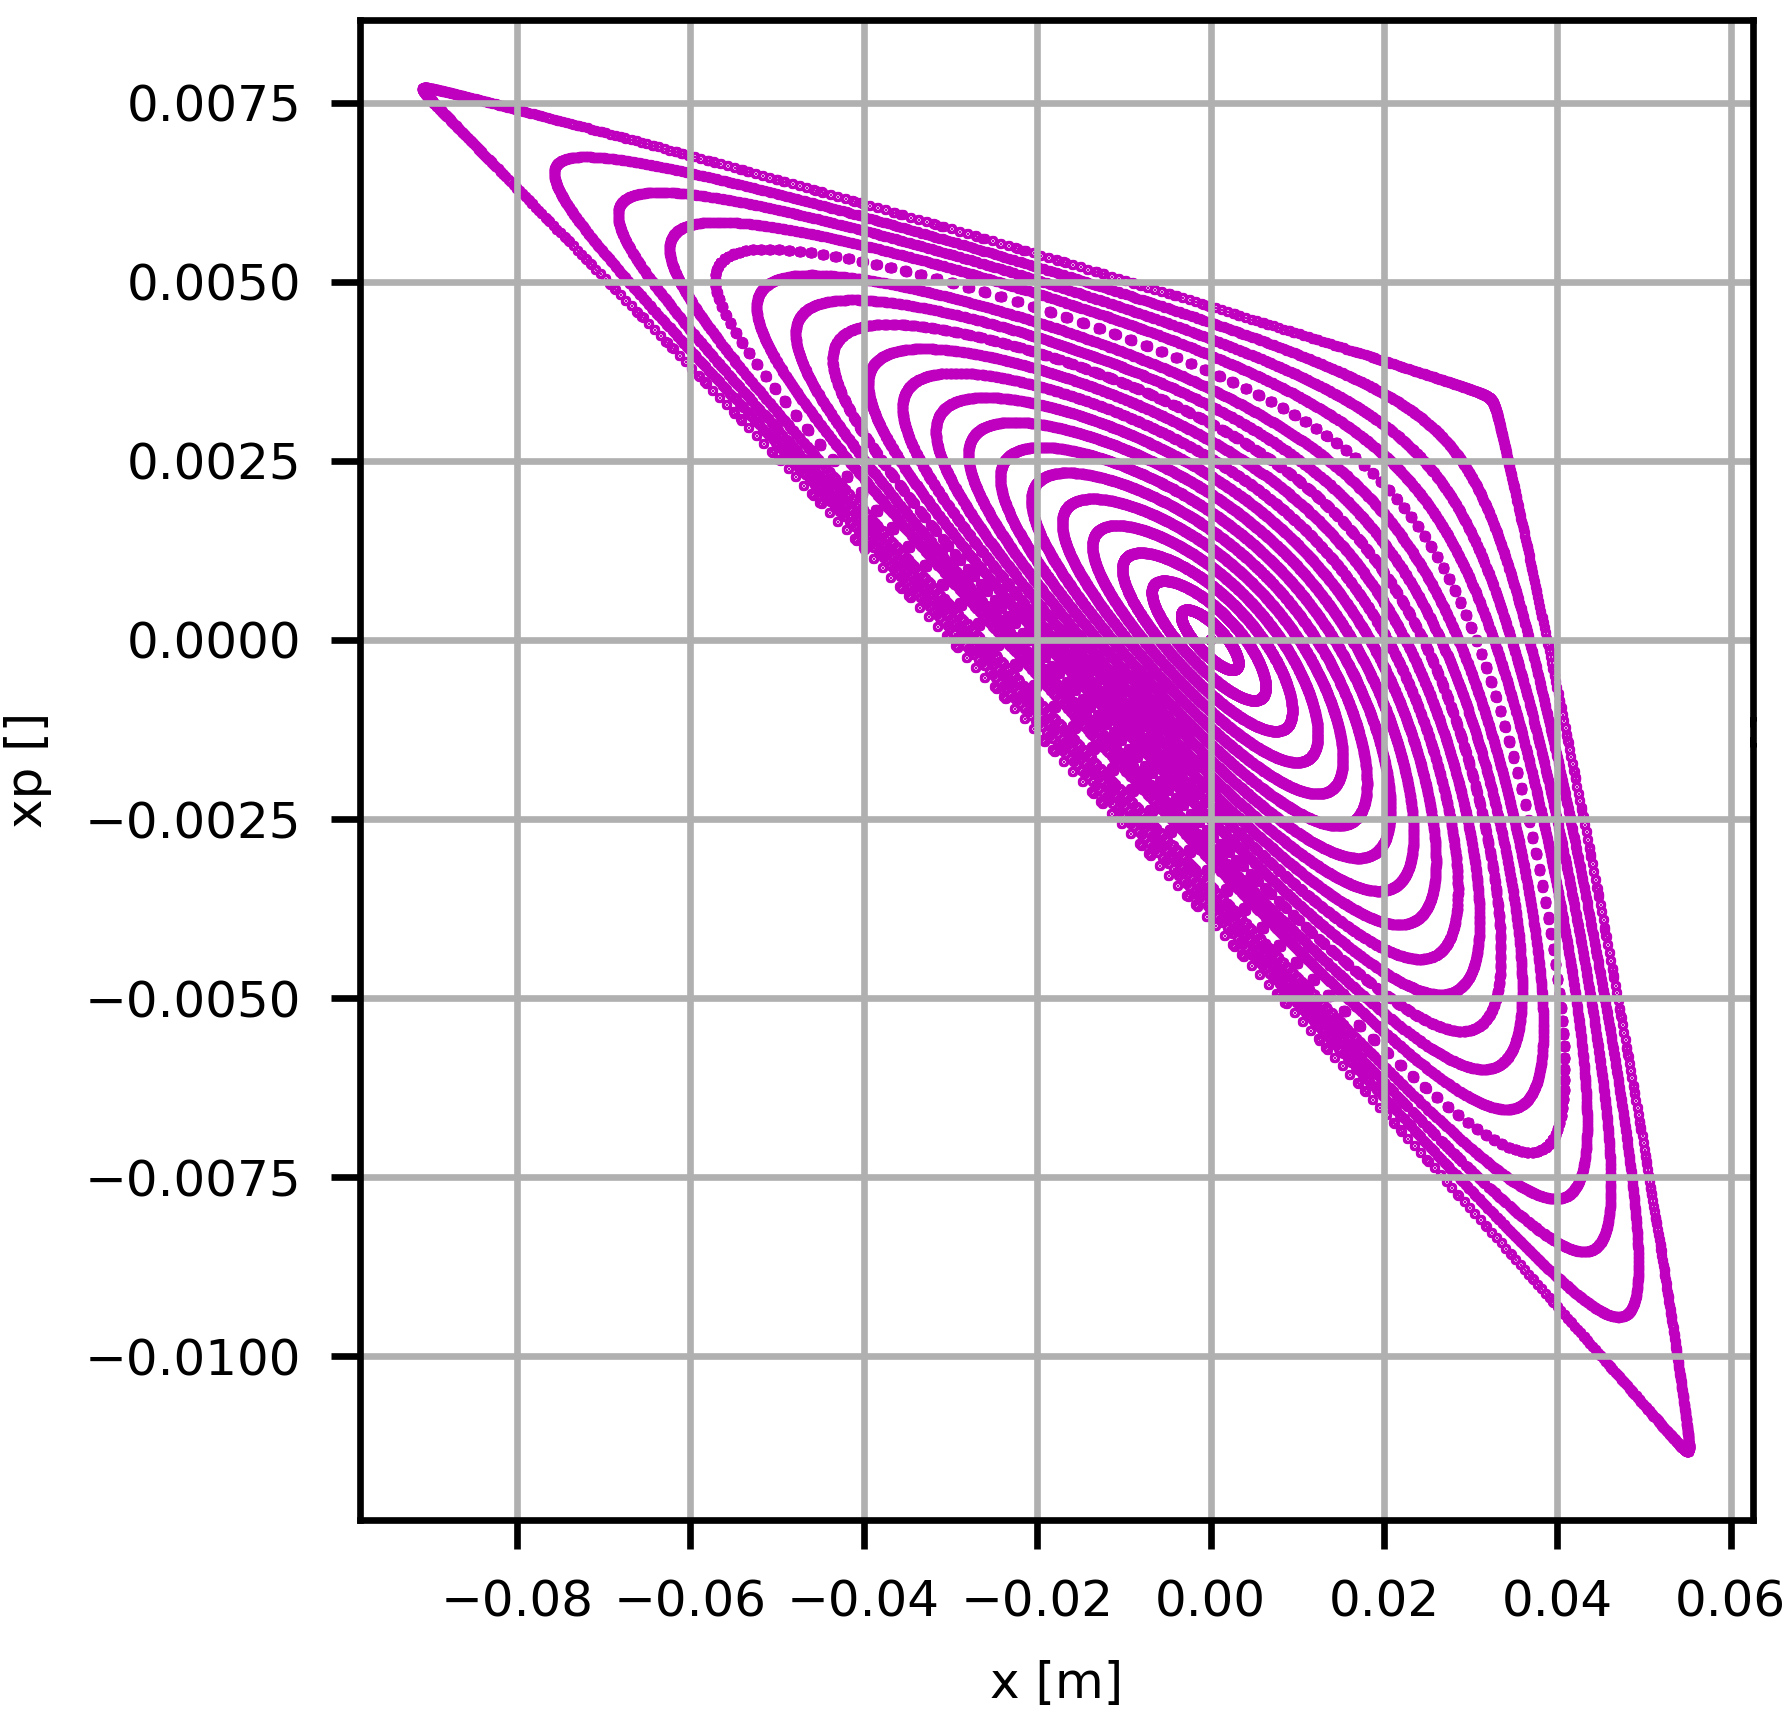
\includegraphics[width=\textwidth]{Step1_phase-space_PO.png}
          \caption{PTC-PyORBIT.}
          \label{fig:step1_po}
        \end{subfigure}
        \caption{Step1: Phase space with sextupole on and no space charge.}
        \label{fig:step1}
\end{figure}




\section{Step 2: Tunes with sextupole off}


\begin{figure}
        \centering
        \begin{subfigure}{.5\textwidth}
          \centering
          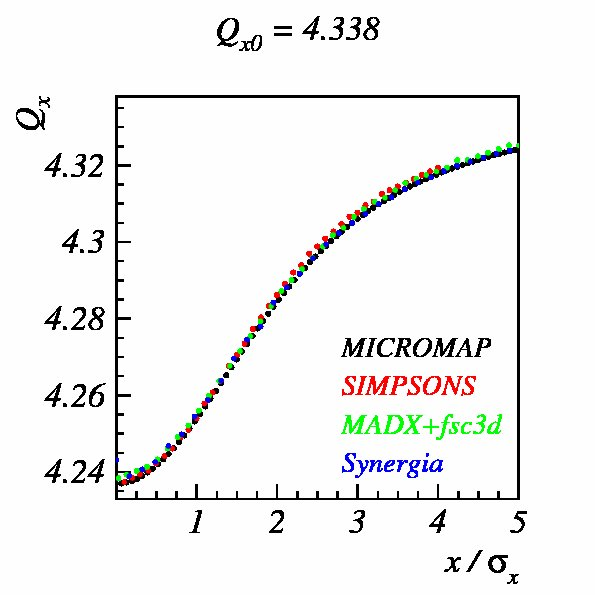
\includegraphics[width=\textwidth]{Step2_tune_x.png}
          \caption{MICROMAP and SIMPSONS.}
          \label{fig:step2_m}
        \end{subfigure}~~~~~~
        \begin{subfigure}{.5\textwidth}
          \centering
          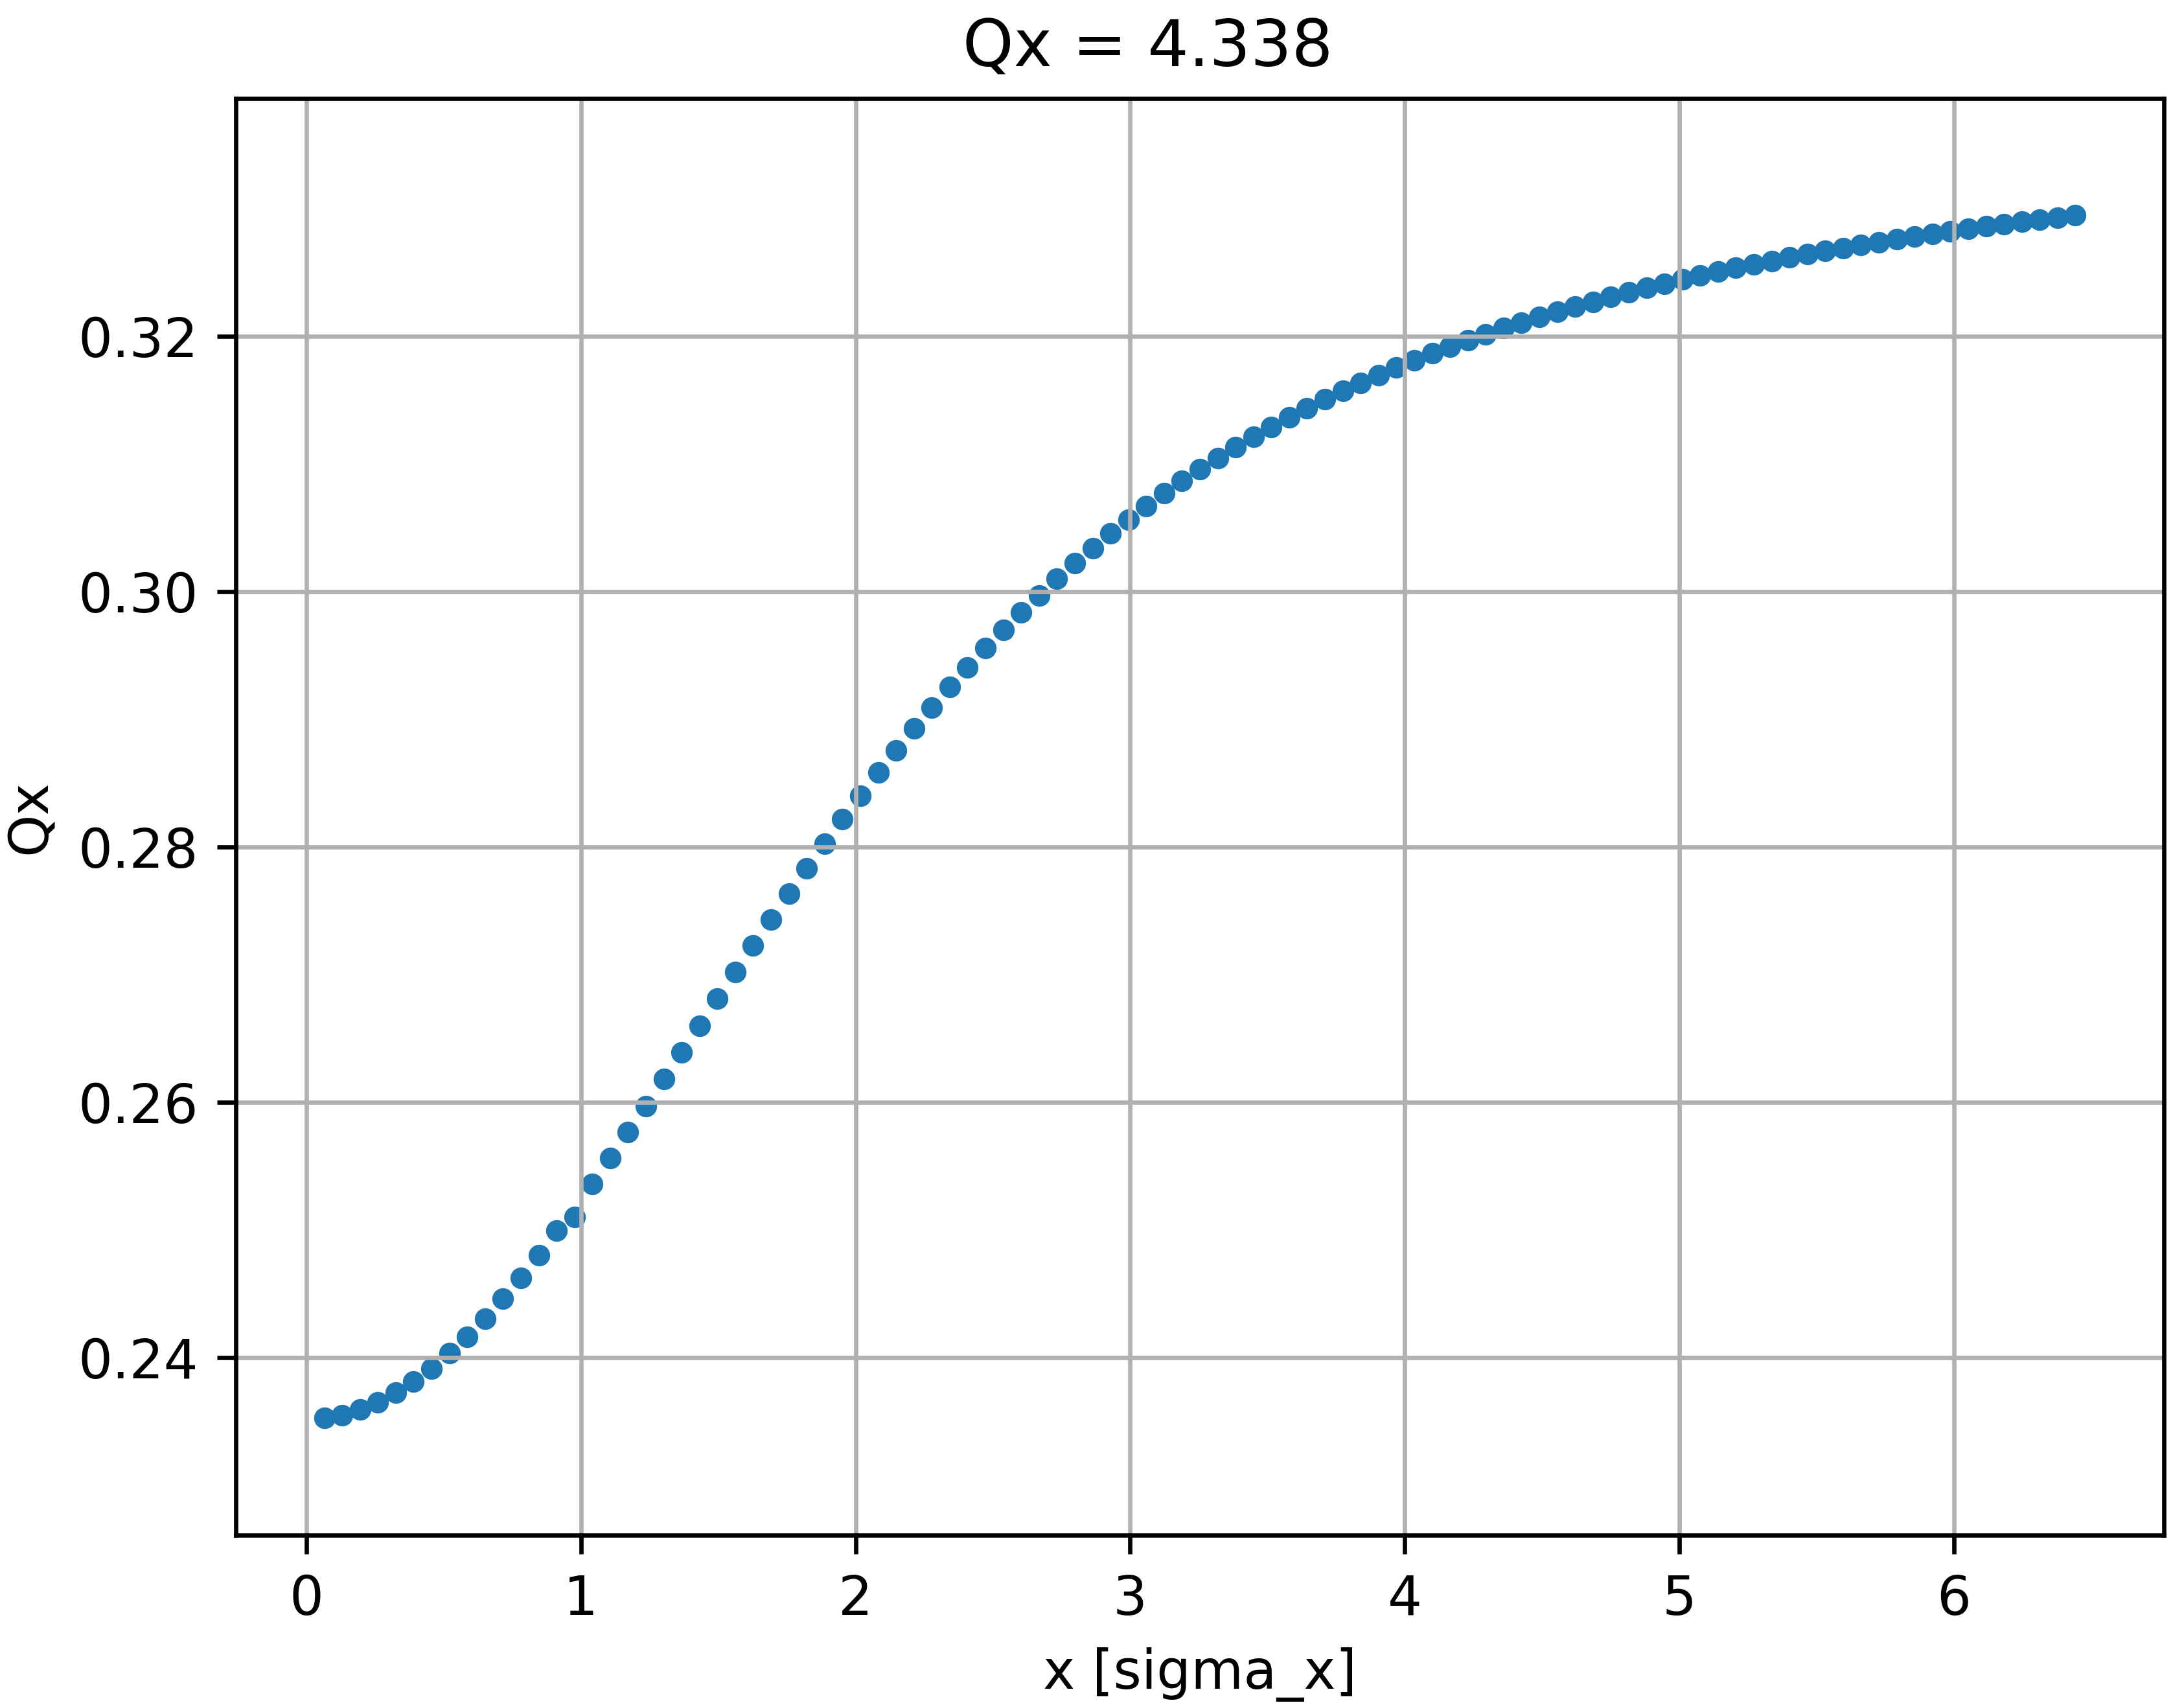
\includegraphics[width=\textwidth]{Step2_tune_x_PO.png}
          \caption{PTC-PyORBIT.}
          \label{fig:step2_po}
        \end{subfigure}
        \caption{Step2: Tune with space charge.}
        \label{fig:step2}
\end{figure}

\begin{figure}[!htb]
        \centering
        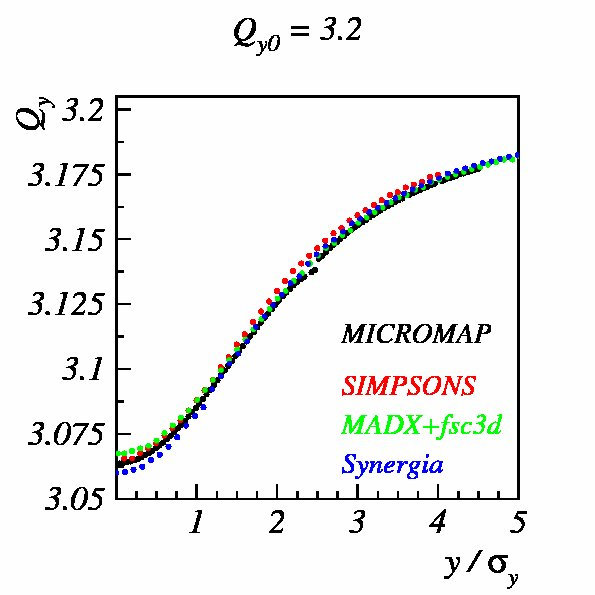
\includegraphics[width=0.5\columnwidth]{Step2_tune_y.jpg}
        \caption{Step2.}
        \label{fig:step2_y}
\end{figure}

\section{Step 3: Tunes with sextupole on at $Q_x$ = 4.338}


\begin{figure}[!htb]
        \centering
        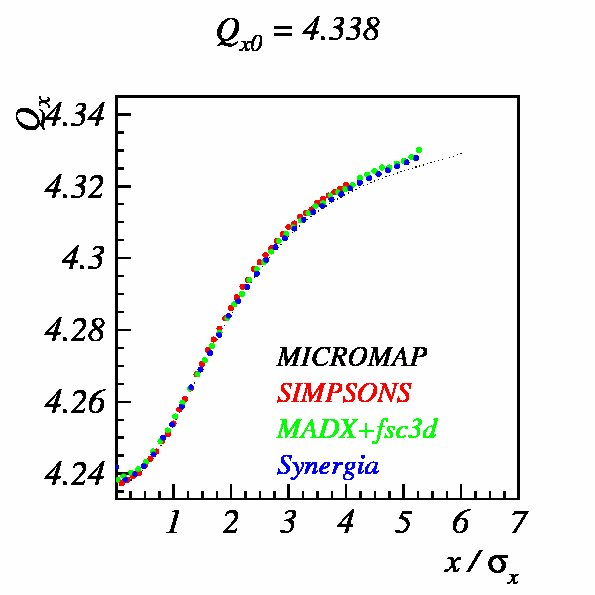
\includegraphics[width=0.5\columnwidth]{Step3_tune_x.jpg}
        \caption{Step3.}
        \label{fig:step3_x}
\end{figure}

\begin{figure}[!htb]
        \centering
        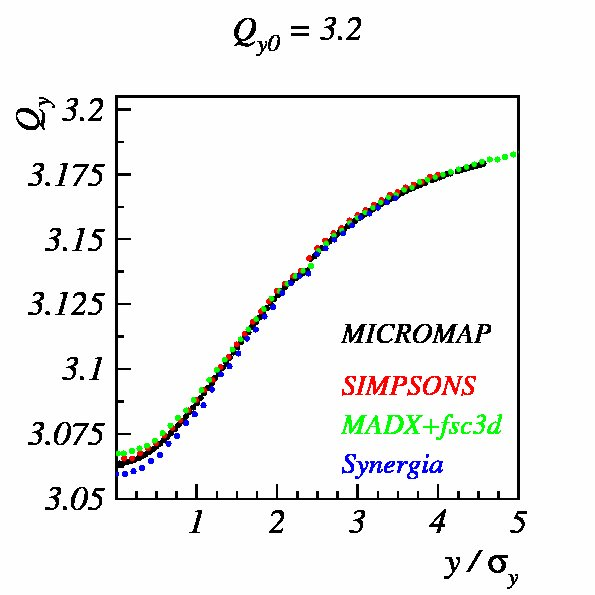
\includegraphics[width=0.5\columnwidth]{Step3_tune_y.jpg}
        \caption{Step3.}
        \label{fig:step3_y}
\end{figure}

\section{Step 4: Tunes with sextupole on at $Q_x$ = 4.3504}

\begin{figure}[!htb]
        \centering
        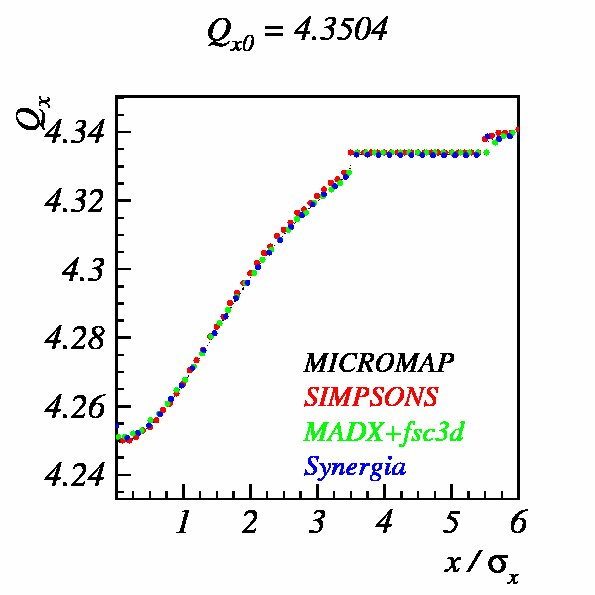
\includegraphics[width=0.5\columnwidth]{Step4_tune_x.jpg}
        \caption{Step4.}
        \label{fig:step4_x}
\end{figure}

\begin{figure}[!htb]
        \centering
        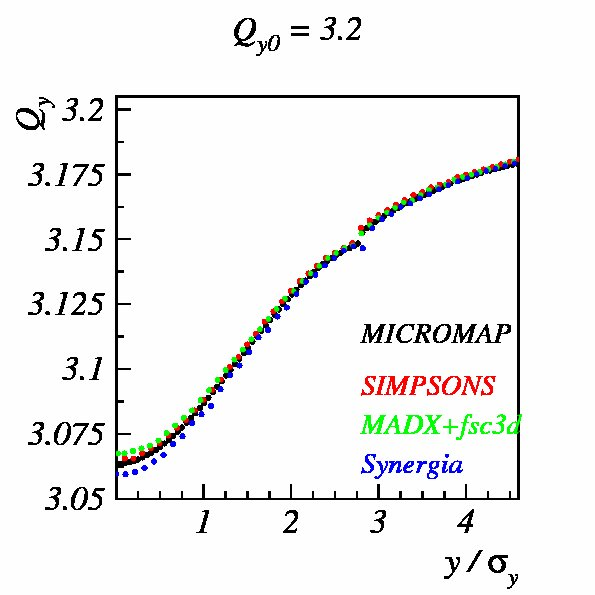
\includegraphics[width=0.5\columnwidth]{Step4_tune_y.jpg}
        \caption{Step4.}
        \label{fig:step4_y}
\end{figure}

\section{Step 5: Phase space with space charge and sextupole on at $Q_x$ = 4.3504}

\begin{figure}[!htb]
        \centering
        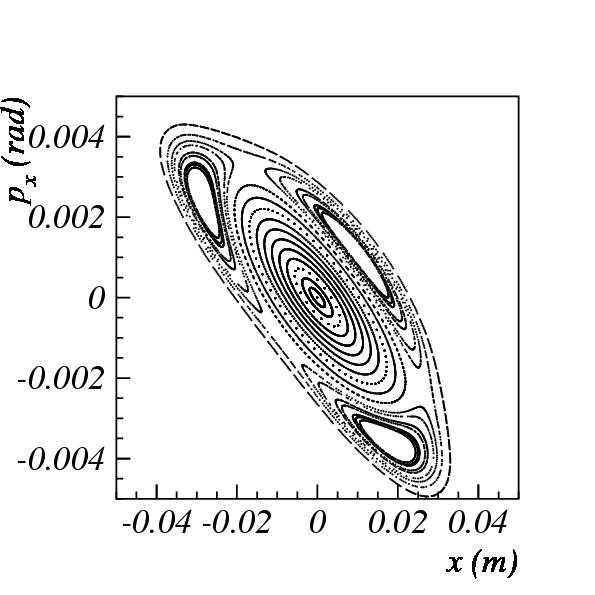
\includegraphics[width=0.5\columnwidth]{Step5_phase-space.jpg}
        \caption{Step5.}
        \label{fig:step5}
\end{figure}

\section{Step 6: Benchmarking of trapping in 1 synchrotron oscillation for $Q_s$ = 1/15000}

\begin{figure}[!htb]
        \centering
        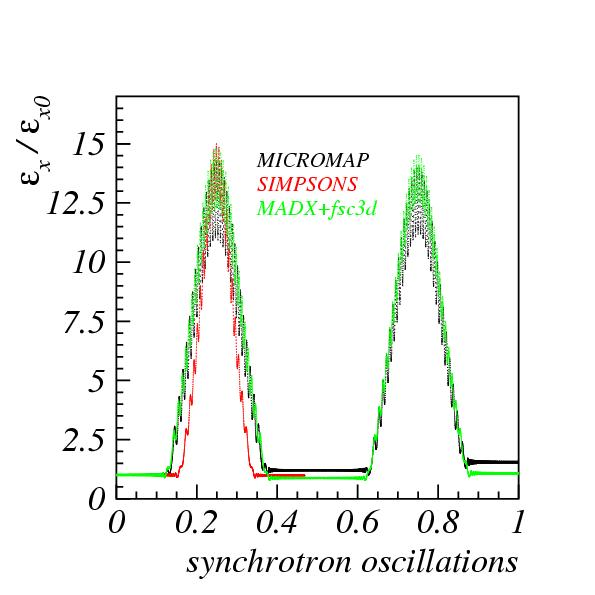
\includegraphics[width=0.5\columnwidth]{Step6_trapping.jpg}
        \caption{Step6.}
        \label{fig:step6}
\end{figure}

\section{Step 7: Benchmarking of trapping in 1 synchrotron oscillation for $Q_s$ = 1/1000}

\begin{figure}[!htb]
        \centering
        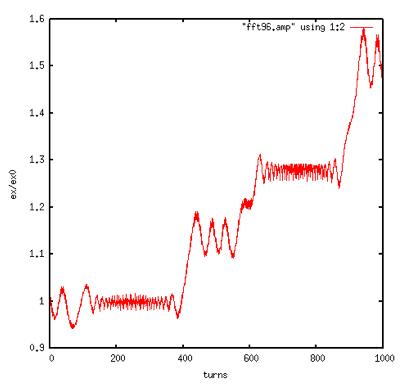
\includegraphics[width=0.5\columnwidth]{Step7_trapping_MICROMAP.jpg}
        \caption{Step7.}
        \label{fig:step7_m}
\end{figure}

\begin{figure}[!htb]
        \centering
        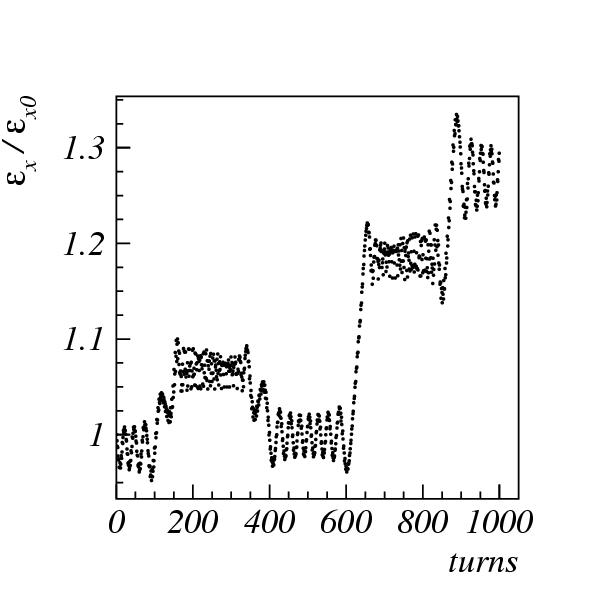
\includegraphics[width=0.5\columnwidth]{Step7_trapping_SIMPSONS.jpg}
        \caption{Step7.}
        \label{fig:step7_s}
\end{figure}

\section{Step 8: Benchmarking of trapping in $5 \cdot 10^5$ turns for $Q_s$ = 1/1000}

\begin{figure}[!htb]
        \centering
        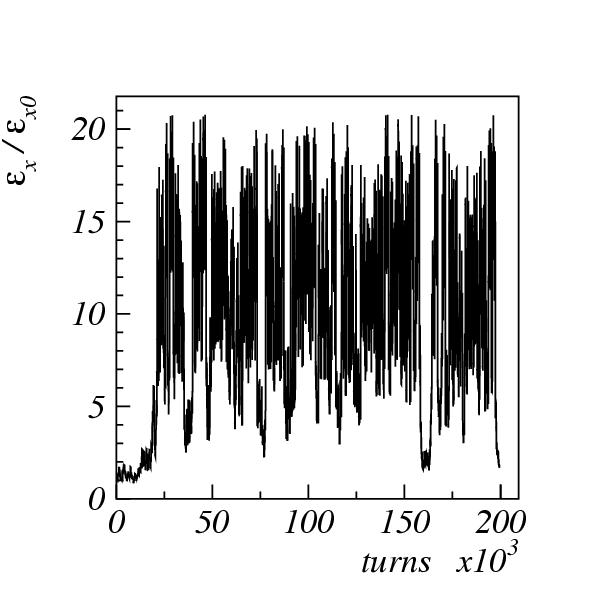
\includegraphics[width=0.5\columnwidth]{Step8_trapping_MICROMAP.jpg}
        \caption{Step8.}
        \label{fig:step8_m}
\end{figure}

\begin{figure}[!htb]
        \centering
        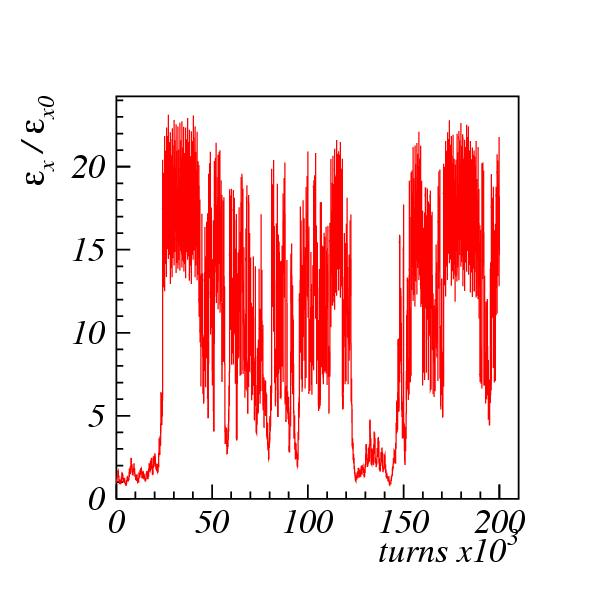
\includegraphics[width=0.5\columnwidth]{Step8_trapping_SIMPSONS.jpg}
        \caption{Step8.}
        \label{fig:step8_s}
\end{figure}

\section{Step 9: Benchmarking of RMS $\epsilon_x$ evolution in $5 \cdot 10^5$ $Q_s$ = 1/1000 for $Q_x$ = 4.3604}

\begin{figure}[!htb]
        \centering
        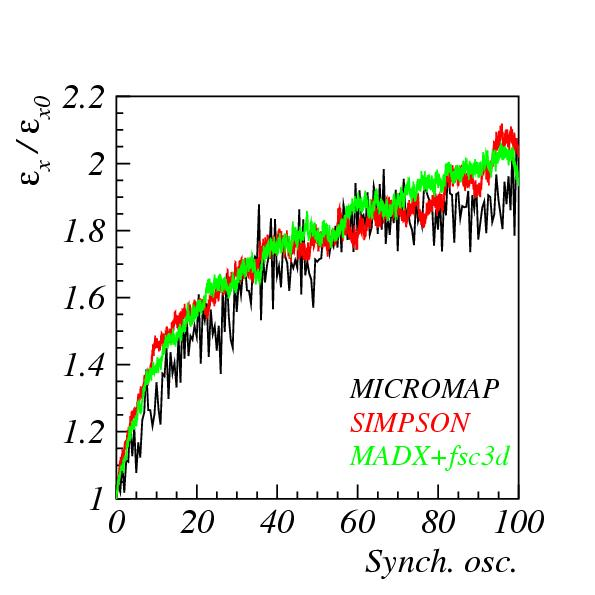
\includegraphics[width=0.5\columnwidth]{Step9_emittance.jpg}
        \caption{Step9.}
        \label{fig:step9}
\end{figure}

\end{document}
